\chapter{面向初学者的拼音键盘设计}
	\section{设计初衷}

  对于中国大陆的儿童来说,初级中文教育并不会详细解释如单元音和复元音等等复杂的概念,儿童对韵母构成的理解局限于整体拼写和读音的一一对应关系。而现阶段的拼音输入法都是基于拉丁字母,对尤其是韵母部分,输入时需要进行拆分,如将 “iang” 拆分为 “i”,“a”,“n”,“g” 进行输入。这相当于要求儿童学习拉丁字母以及基于拉丁字母的键盘,对学习拼音输入的儿童来说是一种负担。

	对于国内的一些中老年人,学习中文的时候,并没有掌握学习拼音。对他们来说,复杂的拉丁字母组合也是学习拼音输入一大难题。这一部分用户使用手写输入法为主,会遇到第\ref{sec:writing}节提到过的问题。尤其考虑到一部分半文盲用户,只具备汉语的听、说、辨识能力,还不具备正确的书写能力,学习拼音输入对他们来说更是难上加难。

	对身居海外的华侨子女,外国人来说,他们学习中文的条件和工具很有限,也是使用的笔画输入法为主。学习使用拼音输入法对他们来说很吃力,将拼音,尤其是韵母拆分为数个拉丁字母进行输入,是一种不直观而且回忆式操作门槛相对较高的方式。特别对有英文输入基础的人,QWERTY键盘反而会有一定程度上的误导性。

	本设计主要面向以上特定人群,⽬的在于克服目前技术中存在的问题,提供⼀种自然的、⾮记忆的中⽂输⼊方法,综合运⽤用汉字多种特征编码,从⽽有效地减少学习负担,提高中⽂输入的效率。当然,对于已经有一定汉语基础,能够熟练掌握汉字声形的用户群体,本设计并不适用。

  此外,考虑到多点触控设备发展迅速,其尺寸有日益增大的趋势,为多点触控等交互手段提供了足够的操作空间。而目前主流拼音输入法中,并没有利用这一优势。本设计希望能充分利用大型触摸设备上多点触控的优势,同时不摒弃原来单点触控的输入方式,提供一种更灵活方便的输入体验。

	\section{设计分析}

	为了达成设计初衷,本设计采用了声母韵母分离独立输入的方式。

	\begin{figure}[h]
	\noindent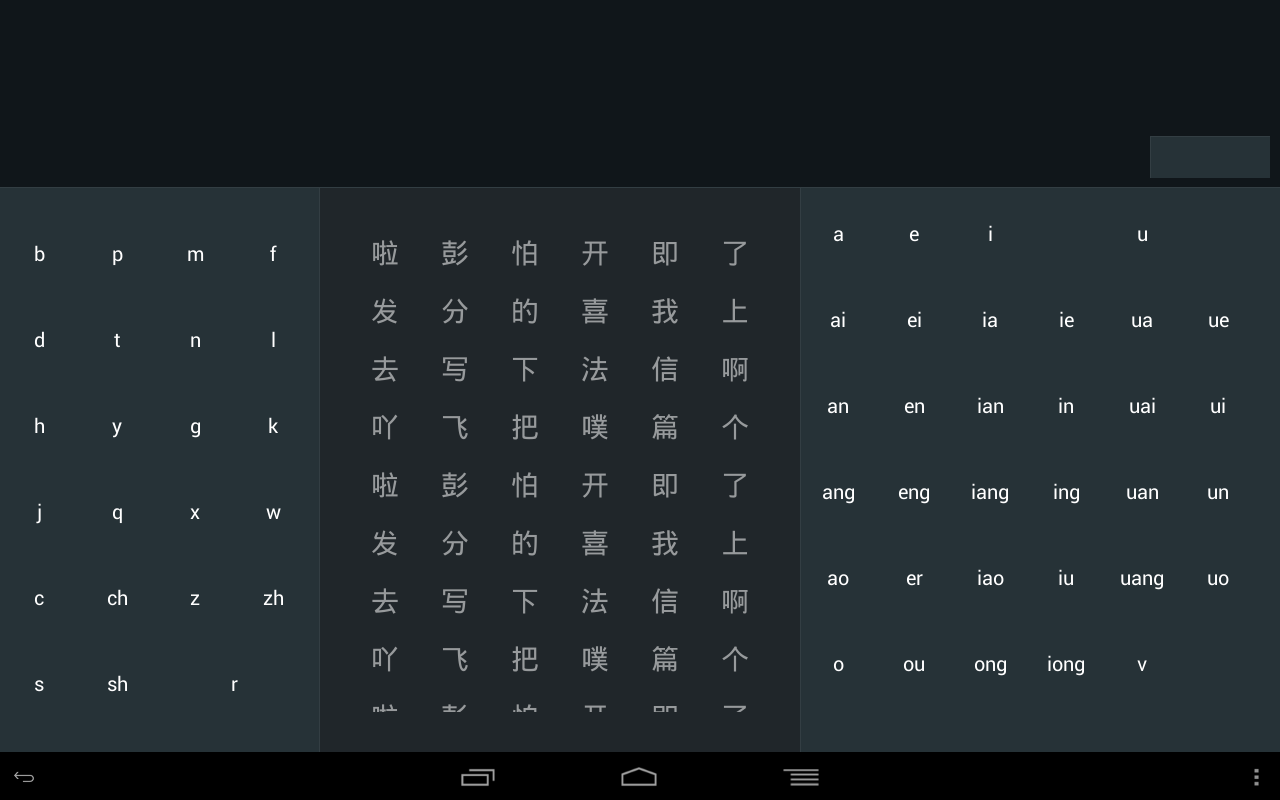
\includegraphics[width=150mm]{img/layout1_background}
	\caption{输入界面}
	\label{fig:layout1_background}
	\end{figure}

	所述检索信息包括声母和韵母中的一项或多项

	所述输⼊设备根据所述检索信息得到各个候选字集后通过设定的算法将所述候选字集整合为最终候选字集,⽤户从所述最终候选字集选择⽬目标汉字输入。最常见的一种算法就是取各个候选字集的交集。

	在本发明的方法中,⽤户可以依次输⼊所述各项检索信息。此时,用户输入一项检索信息后,所述显⽰屏显示根据该检索信息检索得到的候选字集和根据上一项检索信息检索得到的候选字集通过所述设定的算法整合后的候选字集,即显⽰屏上显示的汉字根据用户的输入而更新。

	在本发明的方法中,用户也可以同时输入所述各项检索信息,⽐如,通过多点触控触摸屏同时输入。

	为了提高⽤户的输入效率,考虑到声母和韵母之间并⾮任意搭配,⽽是存在一定的 匹配性,比如,声母 “m” 和韵母 “ia” 就⽆法搭配。因此,在本发明方法中,当用户在声母和韵母中仅输入其中⼀项(即只输⼊声母或只输入韵母)时,所述输⼊设备突出显⽰和⽤户输⼊的声母或韵母相匹配的韵母或声母,便于⽤户输入。此时,若⽤户输⼊未突出显示的韵母或声母,则可以确定⽤户选择的拼音⽆法获得对应的汉字,则认为用户取消了前一次的输⼊,以当前输⼊的声母或者韵母作为初始的拼⾳输入。

	\section{具体实现}

